\chapter{Elektronik}
\label{chap:elektronik}

\section{Schrittmotoren}
Für diesen Prototypen kommen drei Schrittmotoren zum Einsatz.
Einer der Motoren wird als Antrieb der Ziel-Scheibe verwendet und die anderen beiden als Aktuator zum präzisen Positionieren.
Dadurch sind Schrittmotoren sehr interessant für diese Arbeit und werden im folgenden näher erläutert.


\subsection{Funktionsweise}
Schrittmotoren sind Synchronmotoren, welche eine Umdrehung in mehrere Schritte unterteilen.
Diese Schrittunterteilung wird durch Einkerbungen am Stator und am Rotor erreicht.
Eine übliche Schrittweite ist, um ein Beispiel zu nennen, $1,8^\circ$ pro Schritt.
Dadurch eignen sich diese Motoren sehr gut zur sensorlosen Positionierung.
Vorsicht ist jedoch bei zu hohen Drehmomenten oder zu schneller Ansteuerung geboten, da dadurch ein Schrittverlust auftreten kann, welcher sich als Fehler in der Positionierung wiederspiegelt.

Schrittmotoren können wiederum in verschiedene Klassen unterteilt werden.
Die hier relevanten Typen sind der Reluktanz-, der Permanentmagnet- und der Hybrid-Schrittmotor.
Bei dem Permanentmagnet-Schrittmotor ist der Rotor magnetisiert.
Dabei sind die Zähne abwechselnd als Nord- und Südpole ausgeführt.
Bei dem Reluktanz-Schrittmotor besteht der Rotor aus einem weichmagentischen Material.
Daher muss der gesamte magnetische Fluss durch den in den Windungen fließenden Strom erzeugt werden.

Der Hybrid-Schrittmotor ist eine Mischform, bei der versucht wird, die positiven Eigenschaften zu vereinen.
Dabei wird eine höhere Genauigkeit und mehr Drehmoment erzielt. 
Der Rotor wird aus einem Permanentmagneten, welcher in axialer Richtung magnetisiert ist, und gezahnten Weicheisenkränzen aufgebaut. \cite[28]{book:werkzeugmaschinen}

In Abbildung~\ref{img:stepper} ist der Aufbau eines Permanentmagnet-Schrittmotors mit einer Schrittweite von $90^\circ$ dargestellt.

\begin{figure} \centering
	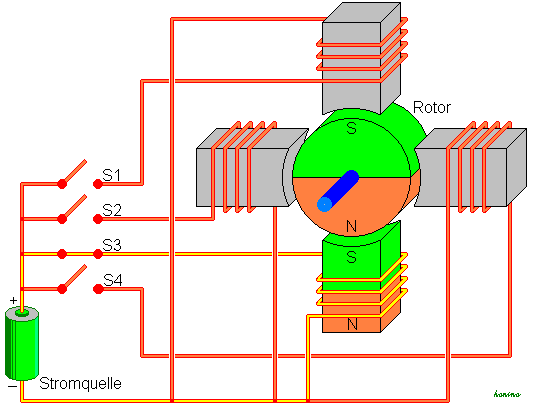
\includegraphics[width=0.5\textwidth]{img/Wikipedia/SchrittmotorUnipolar.PNG}
	\caption{Aufbau eines Schrittmotors mit unipolarer Beschaltung. Quelle: Wikipedia \cite{web:schrittmotor}}
	\label{img:stepper}
\end{figure}


\subsection{Eingesetzte Schrittmotoren}
In diesem Prototypen werden zwei Modelle von Schrittmotoren verwendet.
Der erste Schrittmotor ist jener, welcher zum Antrieb der Scheibe mit den Fotodetektoren verwendet wird.
Dieser benötigt 24 Schritte pro Umdrehung und hat somit einen Schrittwinkel von $15^\circ$.
Bei diesem Schrittmotor ist eine Mittelpunktanzapfung der Spulen vorhanden und somit wäre ein unipolarer Betrieb möglich.
Da bei diesem Schrittmotor jedoch eine, für einen Schrittmotor, hohe Geschwindigkeit erreicht werden soll, wird eine bipolare Beschaltung verwendet.

Der in der Laserablenkeinheit verwendete Schrittmotor ist ein 28BYJ-48 mit einer unipolaren Beschaltung.
Dieser benötigt 64 Schritte pro Umdrehung und besitzt somit einen Schrittwinkel von $5,625^\circ$.
Zusätzlich ist in diesem Motor ein Getriebe mit einem Übersetzungsverhältnis von 64:1 eingebaut.
Nach dem Getriebe hat dieser Motor einen effektiven Schrittwinkel von $0,0879^\circ$.
Dies ist bereits eine feine Unterteilung einer Umdrehung, welche für die Anwendung gerade ausreichend ist.

Zur Verdeutlichung wird mit Gleichung~\ref{equ:posOfLaser} der minimalen Abstand zweier möglicher Positionen eines Laserpunktes berechnet.
Diese maximale Auflösung kann genau dann erreicht werden, wenn der Laser senkrecht zur Grundplatte ausgestrahlt wird.
Dafür wird angenommen, dass die Projektionsfläche 20~cm entfernt ist.
\begin{equation}
a=20~cm \cdot ( tan(90^\circ-2 \cdot (45^\circ + 0.0879^\circ)) - tan(90^\circ-2 \cdot (45^\circ)))
\end{equation}
\begin{equation}
a=20~cm \cdot tan(2 \cdot 0.0879^\circ) = 0,61mm
\end{equation}
Mit dieser Auflösung lässt sich der Laserpunkt genau positionieren.
Eine noch feinere Unterteilung einer Umdrehung würde keinen Mehrwert bringen.
Der limitierende Faktor liegt, bei einer solch feinen Unterteilung, bei dem Spiel der Zahnräder und der Lagerung des Getriebes.
Bei den verwendeten Motoren ist sowohl die Lagerung als auch das Getriebe aus Kunststoffteilen gefertigt.
Möchte man die erzielbare Genauigkeit verbessern, dann kann man dies dadurch erreichen, dass auf ein spielarmes Metallgetriebe umgestiegen wird.


\subsection{Ansteuerung}
Für die Ansteuerung eines Schrittmotors sind zwei Techniken verbreitet.
Diese sind die unipolare und die bipolare Beschaltung.

Bei der unipolaren Ansteuerung ist für jeder Windung eine Mittelpunktanzapfung vorhanden, welche zusätzlich aus dem Motor herausgeführt wird.
Dadurch ist es möglich diesen Mittelpunkt auf Versorgungsspannung zu legen und mit einem Schalter eine der beiden Hälften zu aktivieren.
Der Vorteil dabei ist, dass nur ein schließender Schalter verwendet werden muss.
Es ist also keine Richtungsumkehrung des Stromes notwendig.
Der gravierende Nachteil ist, dass nur die Hälfte der Spule verwendet wird und somit auch nur das halbe Drehmoment generiert wird.
Der in Abbildung~\ref{img:stepper} dargestellte Schrittmotor ist unipolar beschaltet.

Bei der bipolaren Beschaltung werden die Mittelpunkte nicht aus dem Motor herausgeführt oder nicht verwendet.
Dafür muss allerdings die Stromrichtung vorgegeben werden können.
Es ist somit möglich einen Schrittmotor, welcher für eine unipolare Ansteuerung vorgesehen ist, mit einer bipolaren Ansteuerung zu betreiben.
Umgekehrt ist dies im allgemeinen nicht der Fall, da bei manchen Modellen die Mittelpunkte der Spulen nicht herausgeführt werden.

\subsection{H-Brücke}

\begin{figure} \centering
	\begin{minipage}[t]{\linewidth} \centering
		\begin{circuitikz}
\draw
(0,0) to[battery,l=$V_{\text{}}$] ++(0,4)
++(0,0) -- ++(2,0) coordinate (LT)
%%%  H-bridge 1st leg
(LT) ++(2,-1) node [pnp,scale=1,name=igbt1] {}
++(0,-2) node [npn,scale=1,name=igbt3] {}
(igbt1.E) |- (LT)
(igbt1.C) -- (igbt3.C)
(igbt3.E) |- (0,0)
%%% H-bridge 2nd leg
(LT) ++(7,-1) node [pnp,scale=1,name=igbt2, xscale=-1] {}
++(0,-2) node [npn,scale=1,name=igbt4, xscale=-1] {}
(igbt2.E) |- (LT)
(igbt2.C) -- (igbt4.C)
(igbt4.E) |- (0,0)
%%% Output
(LT) ++(2,-2) node[circ] {} to[short,-o] ++(1.3,0) node[anchor=north] {A}
(LT) ++(7,-2) node[circ] {} to[short,-o] ++(-1.3,0) node[anchor=north] {B}
(LT) ++(3.3,-2) to [L,scale=1,name=l1] ++(2.4,0)
%%% Motor Control
(2,-0.5) rectangle (11,-1.5)
(3,-0.5) |- (igbt1.B)
(3.2,-0.5) |- (igbt3.B)
(10.2,-0.5) |- (igbt2.B)
(10,-0.5) |- (igbt4.B)
%%% Diodes
(LT) ++(2.8,-4) node[circ] {} to [Do,scale=1,name=diode0] ++(0,2) node[circ] {} to [Do,scale=1,name=diode1] ++(0,2) node[circ] {}
(LT) ++(6.2,-4) node[circ] {} to [Do,scale=1,name=diode2] ++(0,2) node[circ] {} to [Do,scale=1,name=diode2] ++(0,2) node[circ] {}
;
\node (note1) at (6,-1) {Motor Control};
\end{circuitikz}

	\end{minipage}
	\caption{Aufbau einer H-Brücke für eine Windung}
	\label{img:hBruecke}
\end{figure}

Um eine Windung eines Schrittmotors sowohl in Vorwärts- als auch in Rückwärtsrichtung betreiben zu können, wird eine so genannte H-Brücke benötigt.
Bei dieser Schaltung werden für beide Anschlüsse der Windung sowohl ein Leistungsschalter zur Versorgung als auch einer zur Masse vorgesehen.
Die Art der Leistungsschalter ist dabei unbedeutend und es können sowohl Bipolartransistoren, MOSFETs als auch andere Schalter wie Relais verwendet werden.
Da es sich bei dem zu schaltenden Aktuator um eine Induktivität handelt, sind zusätzlich Freilaufdioden von der Masse und zu der Versorgungsspannung erforderlich.
Die Freilaufdioden schützen die Leistungsschalter vor der in der Induktivität gespeicherten Energie.

Dieser Aufbau ist mit Bipolartransistoren in Abbildung~\ref{img:hBruecke} dargestellt.
Die dargestellte H-Brücke ist in diesem Fall sowohl mit NPN- als auch mit PNP-Transistoren aufgebaut.
Es ist auch möglich die H-Brücke nur mit npn Transistoren aufzubauen, allerdings benötigt man dazu eine hohe Steuerspannung.
In diesem Prototypen kommt ein L298 als H-Brücke zum Einsatz.


\subsection{Vollschrittbetrieb}

\begin{figure}[!h] \centering
	\begin{minipage}[t]{.5\linewidth} \centering
		\begin{tikzpicture}[->,>=stealth',shorten >=1pt,auto,node distance=3cm,
thick,main node/.style={circle,fill=blue!20,draw,font=\sffamily\Large\bfseries}]

\node[main node] (1) {1 1};
\node[main node] (2) [below left of=1] {-1 1};
\node[main node] (3) [below right of=2] {-1 -1};
\node[main node] (4) [below right of=1] {1 -1};

\path[every node/.style={font=\sffamily\small}]
(1) edge 				node [left] 	{F} (4)
(1) edge [bend right] 	node[left] 	{B} (2)
(2) edge 				node [right] 	{F} (1)
(2) edge [bend right] 	node[left] 	{B} (3)
(3) edge 				node [right]	{F} (2)
(3) edge [bend right] 	node[right] 	{B} (4)
(4) edge 				node [left]	{F} (3)
(4) edge [bend right] 	node[right] 	{B} (1);
\end{tikzpicture}
	\end{minipage}
	\caption{FSM eines Schrittmotors mit Vollschritte.}
	\label{fig:fsmStepperVollschritt}
\end{figure}

Für die Ansteuerung gibt es verschiedene Varianten.
Dabei ist es allerdings nicht von Bedeutung, ob die Beschaltung unipolar oder bipolar erfolgt und ist somit unabhängig davon.

Bei der einfachsten Variante werden immer beide Windungen betrieben und nur das Vorzeichen des Stromflusses gewechselt.
Diese Ansteuerung wird Vollschrittbetrieb bezeichnet und kann mit einer FSM sehr elegant beschrieben werden.
Eine mögliche FSM ist in Abbildung~\ref{fig:fsmStepperVollschritt} dargestellt.
Hier wird als Zustand die Richtungen der Ströme verwendet, wobei 1 für einen Strom in Bezugsrichtung, -1 für einen Strom gegen Bezugsrichtung und 0 für eine stromfreie Windung steht.
Ein Vergleich der Abbildung~\ref{fig:fsmStepperVollschritt} mit der Abbildung~\ref{fig:drehgeberZustaende} verdeutlicht, dass es sich bei dem generierten Signal zur Ansteuerung um ein Quadratur-Signal handelt.

Der Vollständigkeit halber ist anzumerken, dass ein Vollschrittbetrieb auch dadurch erreicht werden kann, dass immer nur eine Spule bestromt wird.
Diese Art von Vollschrittbetrieb wird dadurch gekennzeichnet, dass weniger Leistung benötigt wird aber auch ein kleineres Drehmoment erzeugt wird.
Außerdem sind die Schritte um einen Halbschritt versetzt. \cite[142]{book:elMaschienenAktuatoren}


\subsection{Halbschrittbetrieb}

Die Genauigkeit dieser Ansteuerung lässt sich nun verdoppeln, indem nicht nur die Richtungen der Ströme als Zustände verwendet werden, sondern auch erlaubt wird, maximal eine Spule stromfrei zu schalten.
Dies ist also eine Kombination der beiden Varianten für den Vollschrittbetrieb und wird als Halbschrittbetrieb bezeichnet.
Eine FSM für die Halbschrittansteuerung ist in Abbildung~\ref{fig:fsmStepperHalbschritt} dargestellt.

\begin{figure}[!h] \centering
	\begin{tikzpicture}[->,>=stealth',shorten >=1pt,auto,node distance=3cm,
thick,main node/.style={circle,fill=blue!20,draw,font=\sffamily\Large\bfseries}]

\node[main node] (1) {1 1};
\node[main node] (2) [below left of=1] {0 1};
\node[main node] (3) [below right of=2] {-1 1};
\node[main node] (4) [right of=3] {-1 0};
\node[main node] (5) [right of=4] {-1 -1};
\node[main node] (6) [above right of=5] {0 -1};
\node[main node] (7) [above left of=6] {1 -1};
\node[main node] (8) [left of=7] {1 0};

\path[every node/.style={font=\sffamily\small}]
(1) edge 				node [below] 	{F} (8)
(2) edge 				node [below]	{F} (1)
(3) edge 				node [above]	{F} (2)
(4) edge 				node [above]	{F} (3)
(5) edge 				node [above]	{F} (4)
(6) edge 				node [above]	{F} (5)
(7) edge 				node [below]	{F} (6)
(8) edge 				node [below]	{F} (7)
(1) edge [bend right] 	node [above] 	{B} (2)
(2) edge [bend right] 	node [below] 	{B} (3)
(3) edge [bend right] 	node [below] 	{B} (4)
(4) edge [bend right] 	node [below] 	{B} (5)
(5) edge [bend right] 	node [below] 	{B} (6)
(6) edge [bend right] 	node [above] 	{B} (7)
(7) edge [bend right] 	node [above] 	{B} (8)
(8) edge [bend right] 	node [above] 	{B} (1)
;
\end{tikzpicture}
	\caption{FSM eines Schrittmotors mit Halbschritte.}
	\label{fig:fsmStepperHalbschritt}
\end{figure}

Die doppelte Genauigkeit ist hier dadurch erkennbar, dass acht statt vier Zustände benötigt werden.
Eine negative Begleiteigenschaft ist ein Verlust an Drehmoment, wenn mit dem gleichen Strom angesteuert wird.
Dies lässt sich dadurch erklären, dass die Hälfte der Schritte nur mit halben Strom durchgeführt werden. \cite[105]{book:elAntriebstechnik}

\subsection{Mikroschrittbetrieb}
\label{chap:elektronik:mikroschrittbetrieb}

Das Prinzip, einen Schritt zu unterteilen, lässt sich nun beliebig oft anwenden.
Dazu wird zwischen je zwei Zuständen ein neuer Zustand eingefügt, bei welchem nicht der maximale Strom verwendet wird, sondern nur ein Bruchteil davon.
Die Stromregelung kann in diesem Fall mit einer PWM durchgeführt werden.
Da sich der Anker bei jedem Schaltvorgang bewegt, können dadurch Geräusche entstehen.
Deshalb sollte die Frequenz hoch genug sein, um von dem menschlichen Ohr nicht mehr wahrgenommen zu werden.

Dieses Prinzip kann beliebig oft durchgeführt werden, bis die Ansteuersignale einem Sinus und einem Kosinus entsprechen.
Ab einer gewissen Schrittteilung wird jedoch keine höhere Genauigkeit mehr erzielt, da die Position Unregelmäßigkeiten aufweist, welche größer als die Schrittweite ist, der so genannte Winkelfehler.
Diese Grenze ist stark abhängig von dem Typ des Schrittmotors, seiner Bauform, seine Verarbeitungsqualität, des Anwendungsbereichs und weiteren Faktoren.
Der Winkelfehler wird unter anderem durch Belastung, Haftreibung und ungenaue Phasenströme verursacht.
Neben der erhöhten Genauigkeit können dadurch auch Drehmomentrippel reduziert werden.
Drehmomentrippel, auch Drehmomentschwankungen bezeichnet, sind Unregelmäßigkeiten im Verlauf des Drehmoments.
Diese sind meistens unerwünscht, da durch diese Drehschwingungen entstehen können.
Dadurch werden Mechanische Teile wie Getriebe mehr als nötig belastet und es kann zu einer erhöhten Geräuschentwicklung kommen.
\cite[30]{book:werkzeugmaschinen}

Die Grenze für den verwendeten Getriebe-Schrittmotor liegt bei dem Halbschrittbetrieb.
Eine Schrittteilung bringt in diesem Fall nur eine ruhigere Umdrehung mit weniger Drehmomentrippel, diese sind hier jedoch ohnehin nicht von besonderer Bedeutung, da kein Drehmoment übertragen werden muss.
Eine genauere Positionierung ist, wie bereits erläutert, wegen dem Spiel des Getriebes auch nicht möglich.
Bei den für den Antrieb verwendeten Motor ist die Grenze für eine sinnvolle Schrittteilung bereits bei dem Viertelschrittbetrieb erreicht.
Da hier die genaue Positionierung nicht erforderlich ist, wird auch ein Halbschrittbetrieb verwendet.
Dies reduziert die Drehmomentrippel im Vergleich zu einem Vollschrittbetrieb und stellt mehr Drehmoment zur Verfügung als ein Viertelschrittbetrieb.

\section{Auswertung der Gabellichtschranken}
Wenn ein Lichtsignal ausgewertet werden soll, gibt es neben den Fotowiderständen hauptsächlich die Auswahl, ob Fototransistoren oder Fotodioden verwendet werden sollen.
Dabei sind Fotodioden sowohl schnell als auch linear.
Im Vergleich weisen Fotodioden Grenzfrequenzen bis zu 10~MHz und Fototransistoren bis zu 300~kHz auf. \cite[1199]{book:halbleiterSchaltungstechnik}
Die Ansteuerung mit Fotodioden ist aber aufwändiger als jene mit Fototransistoren.
Deshalb werden bei Lichtschranken oft Fototransistoren verwendet.

\begin{figure} \centering
	\begin{minipage}[t]{.49\linewidth} \centering
		\center
\begin{circuitikz}
\draw (0,2)
	to[R] (2,2)
	to[leD*] (2,0)
	-- (0,0);
\draw(0,2) to[american voltage source] (0,0);

\draw (4,1) node[npn,photo] (trans) {}
	(trans.collector) node[anchor=south] {}
	(trans.emitter) node[anchor=north] {};
\draw(4,2)
	--(4,2)
	to[R,*-o](4,4) node[above]{V};
\draw(4,2)
	to[short,*-o](5,2) node[right]{ADC};
\draw(trans.emitter)
	to[short,-o](4,0) node[ground]{};
\draw(4,2) -- (trans.collector);
\end{circuitikz}

	\end{minipage}
	\caption{Einfache Auswertung eines Fototransistors.}
	\label{img:FototransistorWithPullup}
\end{figure}

Für diesen Anwendungszweck ist die Schaltzeit in den meisten Anwendungsfällen ausreichend und Linearität nicht gefordert.
Um einen Fototransistor auszuwerten genügt, als einfachste Variante, ein Spannungsteiler mit einem Widerstand, wie in Abbildung~\ref{img:FototransistorWithPullup} abgebildet.
Bei dieser Art der Ansteuerung reduziert sich die Grenzfrequenz in den einstelligen kHz Bereich.
Dies ist jedoch für einen Inkrementalgeber, wie er hier verwendet wird, ausreichend.

Das Signal der Fototransistoren ist ein analoges Signal, welches je nach Geschwindigkeit und Qualität der Encoderscheiben einem Rechtecksignal oder auch einem Dreiecksignal ähneln kann.
Dies gilt jedoch nur unter guten Bedingungen.
Ist beispielsweise die Encoderscheibe verschmutzt oder durch die Montage beschädigt worden, wird dadurch die Signalform verzerrt.
Mit einem Mikrocontroller ist jedoch ein Rechtecksignal einfacher auszuwerten.
Um das Signal der Fotodioden digital an den Mikrocontroller zu liefern, ist eine zusätzliche Hardware notwendig.

Diese Aufgabe kann durch einen so genannten Schmitt-Trigger erfolgen.
Dieser digitalisiert das Signal nicht nur, er vermeidet mit einer Hysterese auch, dass durch das Rauschen beim Durchgang der Schaltschwelle ein Prellen entsteht. \cite[307]{book:elektrischeMesstechnik}

\section{Laser-Detektion}
Die Detektion des Laserstrahles ist eine Kernaufgabe bei dieser Arbeit.
Dabei sind mehrere Komponenten notwendig.
Grundsätzlich lässt sich das System in den Laser, den Detektor und seine Ansteuerelektronik unterteilen.
Weil der Laser für ein einfaches Auswertungsverfahren nur ein und ausgeschaltet werden muss, genügt eine Emitterschaltung um den Laser anzusteuern.
Bei dem Messen des Fotostromes einer Diode wird eine Schaltung benötigt, welche den Strom verstärkt.


\subsection{Transimpedanzverstärker}
\label{chap:elektronik:tia}

\begin{figure} \centering
	\begin{circuitikz}[scale=1]
	\draw(5,.5)
	node [op amp] (opamp) {}
	%node A at ($(opamp.+)+(-0.4,0)$)
	%(0,0) node [left] {$U_{we}$}
	%to [R, l=$R_d$, o-*] (2,0)
	%to [R, l=$R_d$, *-*] (opamp.+)
	%to [C, l_=$C_{d2}$, *-] ($(opamp.+)+(0,-2)$) node [ground] {}
	(opamp.+) -| (3,-0.3) node [ground] {}
	(3,0) to [pDo, *-*] (3,1)
	%(opamp.+) [pDo] (opamp.-)
	(opamp.out) |- (5.5,2) to [R, l_=$R$, -] (3,2) |- ($(opamp.-)$)
	(5.5,2) to [short, *-] (5.5,3.2) to [C, l_=$C$, -] (3,3.2) to [short, -*] (3,2)
	(opamp.out) to [short, *-o] (7,.5) node [right] {$U_{out}$};
\end{circuitikz}
	%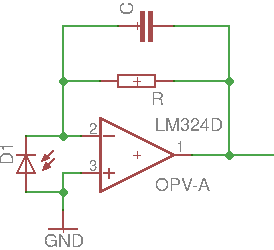
\includegraphics[width=2.5in]{img/Eagle/TIA01.png}
	\caption{Transimpedanzverstärker.}
	\label{fig:transimpedanzverstaerker}
\end{figure}

Fotodioden liefern nur einen kleinen Strom im Bereich von wenigen Mikroampere.
Um mit einem Mikrocontroller diesen Strom präzise messen zu können, ist ein Strom-Spannungs-Wandler notwendig.
Ein so genannter Transimpedanzverstärker (TIA) lässt sich, wie in Abbildung~\ref{fig:transimpedanzverstaerker} dargestellt, mit einem herkömmlichen spannungsgesteuerten Operationsverstärker (VV-OPV) realisieren.
In dieser Beschaltung arbeitet Photodiode wie wenn sie kurzgeschlossen wäre.
Es fällt über die Diode keine Spannung ab.

Eine alternative Beschaltung ist, die Fotodiode nicht gegen Masse sondern gegen eine Vorspannung zu schalten.
Bei dieser Beschaltung würde nicht die Kathode am invertierenden Eingang anliegen, sondern die Anode.
Die Fotodiode wird in dieser Beschaltung in einem anderen Quadranten der Kennlinie betrieben und kann eine höhere Grenzfrequenz erreichen. \cite[80]{book:pulseOximeters} \cite[89]{book:bauelementGrundschaltungen}

Da eine Gegenkopplung vorliegt, sind die Eingänge des OPV mit einem virtuellen Kurzschluss verbunden.
Deshalb ist der Strom durch den Widerstand gleich dem Fotostrom der kurzgeschlossenen Diode.
Die Spannung am Ausgang ist nun die negative Spannung des Widerstandes, da sich die Richtung des Bezugssystemes geändert hat.
Somit ergibt sich die Ausgangsspannung zu:
\begin{equation}
U_a = R * I_R = - R * I_E
\end{equation}
Mit dem Widerstand R lässt sich nun die Spannung am Ausgang einstellen.
In der Praxis wird dieser allerdings experimentell bestimmt, da der einfallende Fotostrom nur unzureichend bekannt ist.
Für diesen Aufbau hat sich ein Widerstand von $R=100~k\Omega$ als optimal erwiesen.

Da die Fotodiode eine parallele Kapazität hat, welche durch die Raumladungszone entsteht, wird eine Phasennacheilung in der Gegenkopplung erzeugt.
Dies kann die Schaltung instabil machen.
Um dem entgegenzuwirken wird ein Kondensator parallel zum Widerstand geschaltet.
Die Größe der Kapazität ist zwar berechenbar, allerdings ist dafür der Wert des Sperrschichtwiderstandes erforderlich.
Dieser wird in den Datenblättern nur selten angeben.
Auch im Fall der verwendeten BPW34 ist dieser im Datenblatt nicht vorhanden.
Deshalb muss die Kapazität, welche im Bereich von wenigen pF liegt, experimentell bestimmt werden.
Für manche Anwendungsfälle sind die vorhandenen Streukapazitäten bereits ausreichend.
Auch bei dem Aufbau dieses Prototypen sind die Streukapazitäten bereits groß genug, um eventuelle Schwingungen in akzeptabler Zeit abklingen zu lassen.

\subsection{Transiente Vorgänge}
\label{chap:elektronik:transienteVorgaenge}

\begin{figure} \centering
	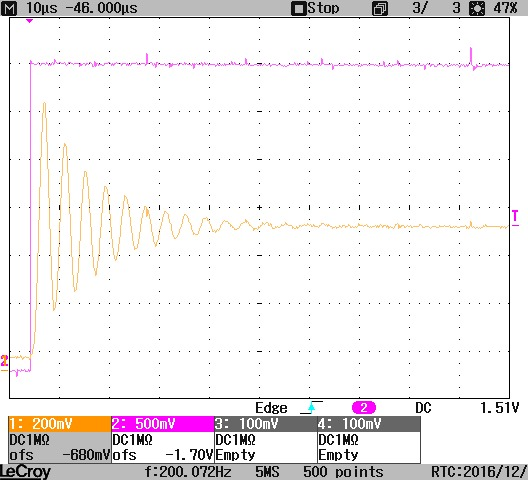
\includegraphics[width=0.49\textwidth]{img/PicturesPlots/Fotodiodes/LaserSchwach/Steigend/COPY/CONVERT/SCRN0132_Cutted.jpg}
	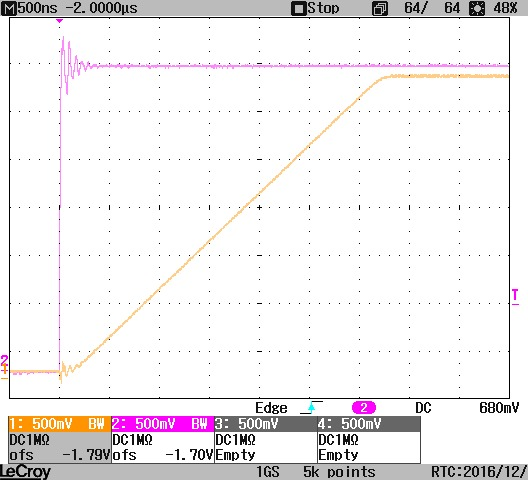
\includegraphics[width=0.49\textwidth]{img/PicturesPlots/Fotodiodes/LaserMaximal/Steigend/COPY/CONVERT/SCRN0088_Cutted.jpg}
	\caption{Abrupter Lichtanstieg bei Transimpedanzverstärker.}
	\label{fig:laserErkennungSteigend}
\end{figure}

\begin{figure} \centering
	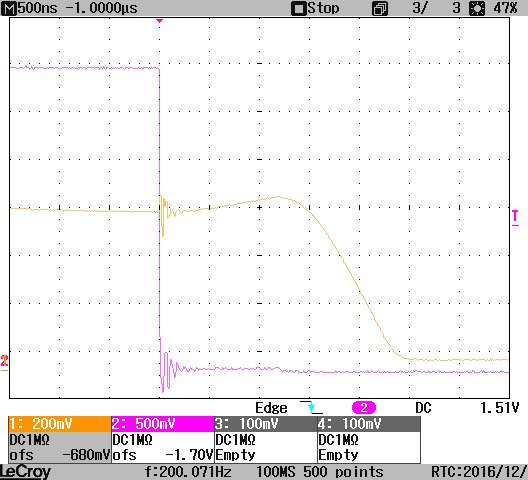
\includegraphics[width=0.49\textwidth]{img/PicturesPlots/Fotodiodes/LaserSchwach/Fallend/COPY/CONVERT/SCRN0135_Cutted.jpg}
	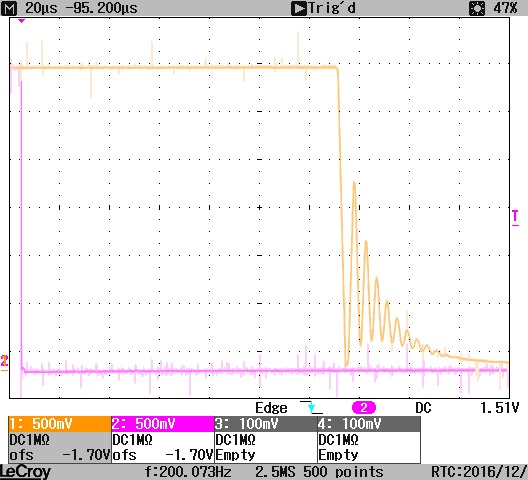
\includegraphics[width=0.49\textwidth]{img/PicturesPlots/Fotodiodes/LaserMaximal/Fallend/COPY/CONVERT/SCRN0142_Cutted.jpg}
	\caption{Abrupter Lichtabfall bei Transimpedanzverstärkers.}
	\label{fig:laserErkennungFallend}
\end{figure}

Bei einem sprungartigen Einschalten des Lasers müssen zuerst die vorhandenen Kapazitäten geladen werden, bevor die korrekte Ausgangsspannung abgreifbar ist.
Da die Fotodiode im Kurzschluss betrieben wird, muss die Sperrschichtkapazität nicht geladen werden. Somit bleibt die Kapazität des TIA übrig.
Dieser Vorgang kann in Abbildung~\ref{fig:laserErkennungSteigend} beobachtet werden.
Im linken Bild fällt nur ein kleiner Teil des Laserlichtes auf die Sensorfläche.
Es ist auch gut ersichtlich, dass bevor sich ein stationärer Endzustand einstellt, die Ausgangsspannung schwingt.
Nach etwa $50~\mu s$ kann der Ausgangswert als stationär angenommen werden.
Im rechten Bild ist der Laser direkt auf die Fotodiode ausgerichtet.
In diesem Fall wird der TIA in die Sättigung gebracht und die Zeit, welche für die transienten Vorgänge benötigt wird, liegt unter $4~\mu s$.
Diese Werte sind wichtig, und müssen später in der Software berücksichtigt werden.

Auch bei den Abschaltvorgängen existieren wieder transiente Vorgänge.
Diese sind in Abbildung~\ref{fig:laserErkennungFallend} abgebildet.
Die Zeiten betragen hier $2,5~\mu s$ und $180~\mu s$.
Interessant ist, dass bei starken Einstrahlung der Einschaltvorgang schneller und der Abschaltvorgang langsamer abläuft.
Diese lange Totzeit ist darauf zurückzuführen, dass sich im Fall einer Sättigung eine Sperrschichtkapazität aufbauen kann, da die Diode nicht mehr im Spannungsnullpunkt betrieben wird.

\subsection{Quadrantendiode}

\begin{figure} \centering
	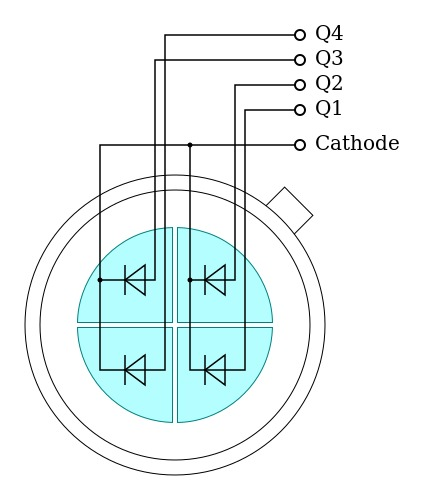
\includegraphics[width=2.5in]{img/Wikipedia/QuadrantenFotodiode.jpg}
	\caption{Quadrantenfotodiode. Quelle: Wikipedia \cite{web:quadrantendiode}}
	\label{fig:quadrantendiode}
\end{figure}

Um nun die Lage eines Laserpunktes bestimmen zu können, werden mehrere Fotodioden benötigt.
Dazu gibt es verschiedene Möglichkeiten diese Fotodioden anzuordnen.
Die bekannteste Variante ist die Quadrantendiode.
Dabei werden vier Fotodioden mit einem kleinen Abstand zwischen den Sensorflächen nebeneinander positioniert.
Die 
In Abbildung~\ref{fig:quadrantendiode} ist eine Quadrantendiode schematisch dargestellt.
Diese können fertig in einem Gehäuse verbaut gekauft werden.
Auch Anordnungen mit mehr als vier Dioden sind erhältlich, sogenannte sedimentierte Fotodioden.

Bei dieser Arbeit werden vier einzelne BPW34 Dioden verwendet.
Für die Schaltung dieses Prototypen kommt eine gemeinsame Anode zum Einsatz, da damit ein OPV mit einer einseitigen Versorgung ausreicht und keine Vorspannung eingestellt werden muss.

\subsection{Auswertung}
\label{chap:elektronik:auswertung}
Um mit der bereits vorgestellten Hardware zu detektieren, wie viel von dem Laserlicht auf die Fläche der Fotodiode fällt, ist ein Algorithmus zur Auswertung notwendig.
Zur Vereinfachung wird angenommen, dass die Ausgangsspannung linear proportional zu dem einfallenden Lichtstrom ist.
Dies ist in der ersten Näherung, wie wir gezeigt haben, auch erfüllt.
Dadurch kann die gemessene Intensität bei eingeschaltetem Laserstrahl von der bei ausgeschaltetem Laserstrahl subtrahiert werden.
Dabei ist allerdings wichtig, dass sich mögliche Störungen langsamer ändern, als die zeitlich Entfernung der Messpunkte.
Da nach dem Einschalten des Lasers, das Ausgangssignal nicht sofort auf den Endwert springt, müssen die in Kapitel~\ref{chap:elektronik:transienteVorgaenge} vermessenen Einschaltvorgänge abgewartet werden.


\subsection{Verbesserte Verfahren}
Eine Verbesserung zu dem bereits vorgestellten Verfahren zur Auswertung der Ausrichtung eines Laserstrahls wäre, den Laserstrahl zu modulieren.
Anstatt nur die auftreffende Intensität mit der Dunkelintensität zu vergleichen, wird ein sinusartiger Lichtstrom erzeugt.
Im Empfänger wird nun mit einem phasenselektiven Synchrongleichrichter (PSSG) oder einem phasenunabhängigen Synchrondemodulator (PUSD) das Signal auf einen bestimmten Frequenzbereich überprüft.
Beide Verfahren stellen schmalbandige Bandpassfilter dar.
Damit lassen sich alle Störungen, welche nicht in der Messfrequenz oder deren Oberschwingungen moduliert sind, unterdrücken.~\cite[210]{book:elektrischeMesstechnik}.

Dazu ist es allerdings notwendig, den Laser auf einem Arbeitspunkt zu modulieren, was mit einer steuerbare Stromquelle realisiert werden kann.
Diese wird mit einem Frequenzgenerator gespeist.
Der Frequenzgenerator ist zum Beispiel durch den DAC des Microcontrollers realisierbar.
Neben dem schaltungstechnisch erhöhten Aufwand wird eine zusätzliche Software auf dem Mikrocontrollers benötigt.
Der wichtigste Nachteil ist allerdings die erhöhte Rechenzeit.
Diese wird benötigt, um das Ausgangssignal zu generieren und eine ausreichend hohe Abtastrate zu erreichen.
Aufgrund der beschränkten Rechenleistung auf dem Mikrocontroller kamen diese Verfahren nicht zum Einsatz.
